\documentclass{article}
\usepackage[utf8]{inputenc}
\usepackage{graphicx}
\usepackage{ragged2e}
\usepackage[margin=2.5cm]{geometry}
\usepackage{array}
\usepackage{wrapfig}
\usepackage{multirow}
\usepackage{tabularx}
\usepackage{amsmath}
\usepackage{wrapfig}
\usepackage{mathtools}
\usepackage[table]{xcolor}
\usepackage{multirow}
\usepackage{polski}
\usepackage{rotating}


\title{Symulacje w Simulink}
\author{AUTOR}
\date{}




\begin{document}
\maketitle
\section{Cel ćwiczenia.}
Nauka rozwiązywania równań różniczkowych przy pomocy modułu Simulink w programie Matlab.  
\section{Schemat blokowy Simulink.}
Równianie dla schematu:
$$
a_1\dot{x}(t)+a_0x(t)=bu(t) \Rightarrow \dot{x}(t)=\frac{1}{a_1}( -a_0x(t)+bu(t))
$$
\begin{figure}[h!]
    \centering
    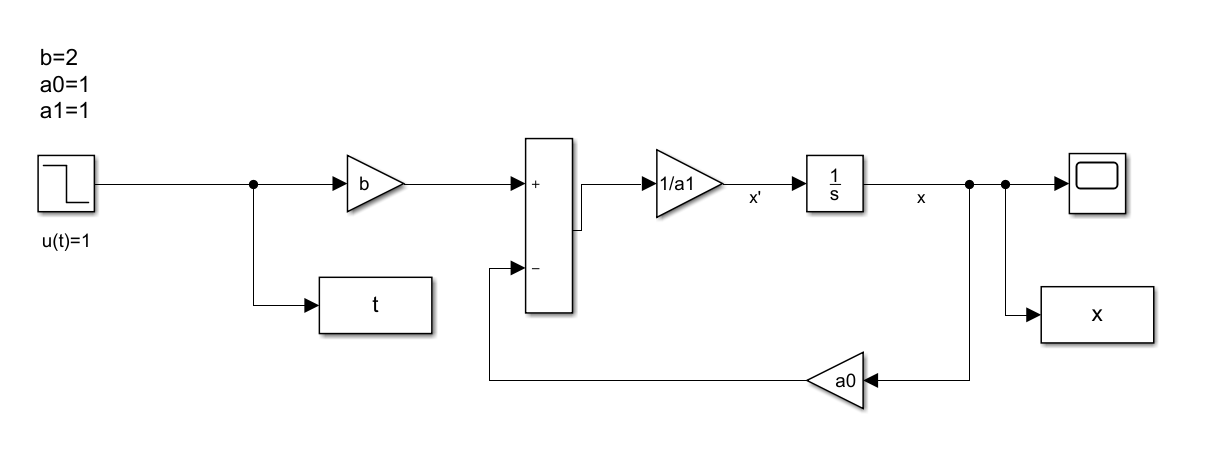
\includegraphics[width=0.985\textwidth]{POPRAWAuklad2.png}
    \label{fig:my_label}
\end{figure}


\newpage
\section{Rozwiązanie - stałe wymuszenie, różne warunki początkowe}
Równanie:
$$
a_1\dot{x}(t)+a_0x(t)=bu(t)
$$
\begin{center}
    $u(t)=1$\\
    $a_0=1$\\
    $a_1=1$\\
    $b=2$\\
\end{center}
Rozwiązanie analityczne:\\
$$\dot{x}(t)+x(t)=2u(t)$$\\
Rozwiązanie swobodne:
$$
\dot{x}_s(t)+x_s(t)=0
$$
$$
x_s(t)=Ae^{\lambda t}, \ \dot{x}_s(t)=\lambda Ae^{\lambda t}
$$
$$
\lambda Ae^{\lambda t}+Ae^{\lambda t}=0/:Ae^{\lambda t}
$$
$$
\lambda+1=0\Rightarrow \lambda=-1
$$
$$
x_s(t)=Ae^{-t} - \text{rozwiązanie swobodne}
$$
Rozwiązanie wymuszone:
$$
\dot{x}_w(t)+x_w(t)=2\cdot1
$$
$$
u(t)=1, \ \dot{u}(t)=0
$$
$$
x_w(t)=C_1\cdot1+C_2\cdot0
$$
$$
x_w(t)=C_1, \ \dot{x}_w(t)=0
$$
$$
C_1=2\Rightarrow x_w(t)=2 -\text{rozwiązanie wymuszone}
$$
Rozwiązanie ogólne:
$$
x(t)=x_s(t)+x_w(t)=Ae^{-t}+2
$$
\begin{flushleft}
    a) Warunek początkowy $\dot{x}(0)=0$
\end{flushleft}
Rozwiązanie analityczne:
$$
x(t)=Ae^{-t}+2 \Rightarrow \dot{x}(t)=-Ae^{-t}
$$
$$
\dot{x}(0)=-A=0\Rightarrow A=0
$$
$$
x(t)=2-\text{rozwiązanie szczególne}
$$
$$
x_s(t)=0, \ x_w(t)=2
$$
Warunek początkowy $\dot{x}(0)=0\Rightarrow x(t)=2 \Rightarrow x(0)=2$\\
Wykres dla rozwiązania analitycznego i symulacyjengo oraz wykres dla rozwiązania analitycznego wraz z składowymi:
\newpage
\begin{figure}[h!]
    \centering
    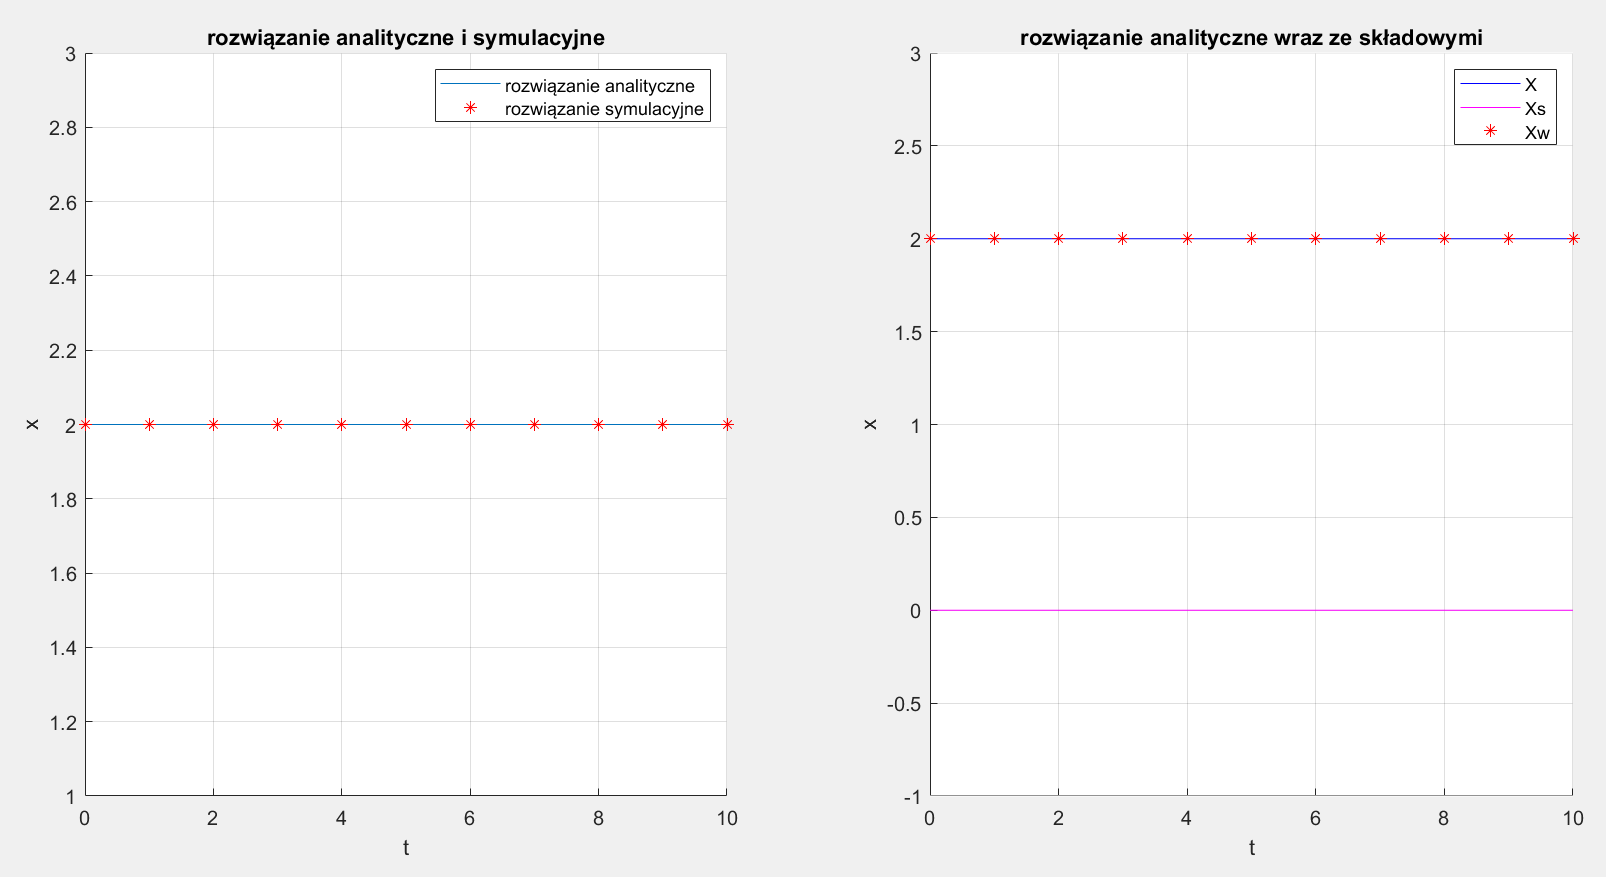
\includegraphics[width=0.985\textwidth]{poprawaBBBBBB.png}
    \label{fig:my_label}
\end{figure}

%$$
%x(0)=2
%$$

b) Warunek początkowy $\dot{x}(0)=4$

Rozwiązanie analityczne i jego wykres wraz z wykresem składowych rozwiązania:
$$
x(t)=Ae^{-t}+2 \Rightarrow \dot{x}(t)=-Ae^{-t}
$$
$$
\dot{x}(0)=-A=4\Rightarrow A=-4
$$
$$
x(t)=-4e^{-t}+2-\text{rozwiązanie szczególne}
$$
$$
x_s(t)=-4e^{-t}, \ x_w(t)=2
$$

Warunek początkowy $\dot{x}(0)=4\Rightarrow x(0)=-4e^{0}+2=-2\Rightarrow x(0)=-2$
Wykres dla rozwiązania analitycznego i symulacyjengo oraz wykres dla rozwiązania analitycznego wraz z składowymi:
\begin{figure}[h!]
    \centering
    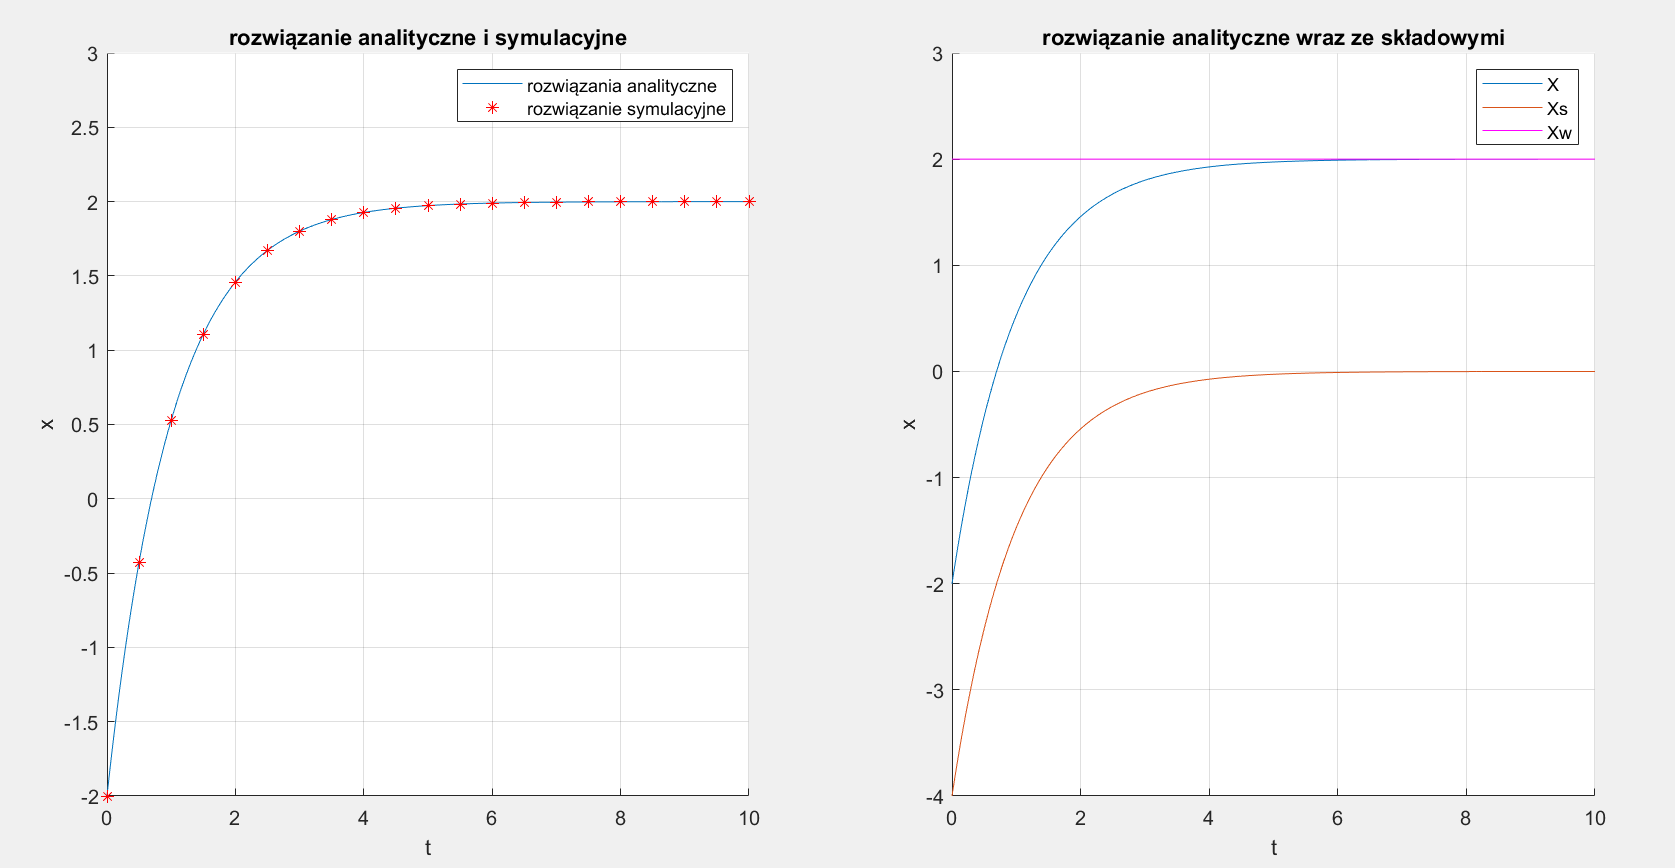
\includegraphics[width=0.928\textwidth]{POPRAWAwykresb.png}
    \label{fig:my_label}
\end{figure}
\\
c) Warunek początkowy $x(0)=0$\\

Rozwiązanie analityczne, jego wykres wraz z wykresem składowych jego rozwiązania:\\
$$
x(t)=Ae^{-t}+2
$$
$$
0=A+2 \Rightarrow A=-2
$$
$$
x(t)=-2e^{-t}+2-\text{rozwiązanie szczególne}
$$
$$
x_s(t)=-2e^{-t}, \  x_w(t)=2
$$
%$$
Wykres dla rozwiązania analitycznego i symulacyjengo oraz wykres dla rozwiązania analitycznego wraz z składowymi:
\begin{figure}[h!]
    \centering
    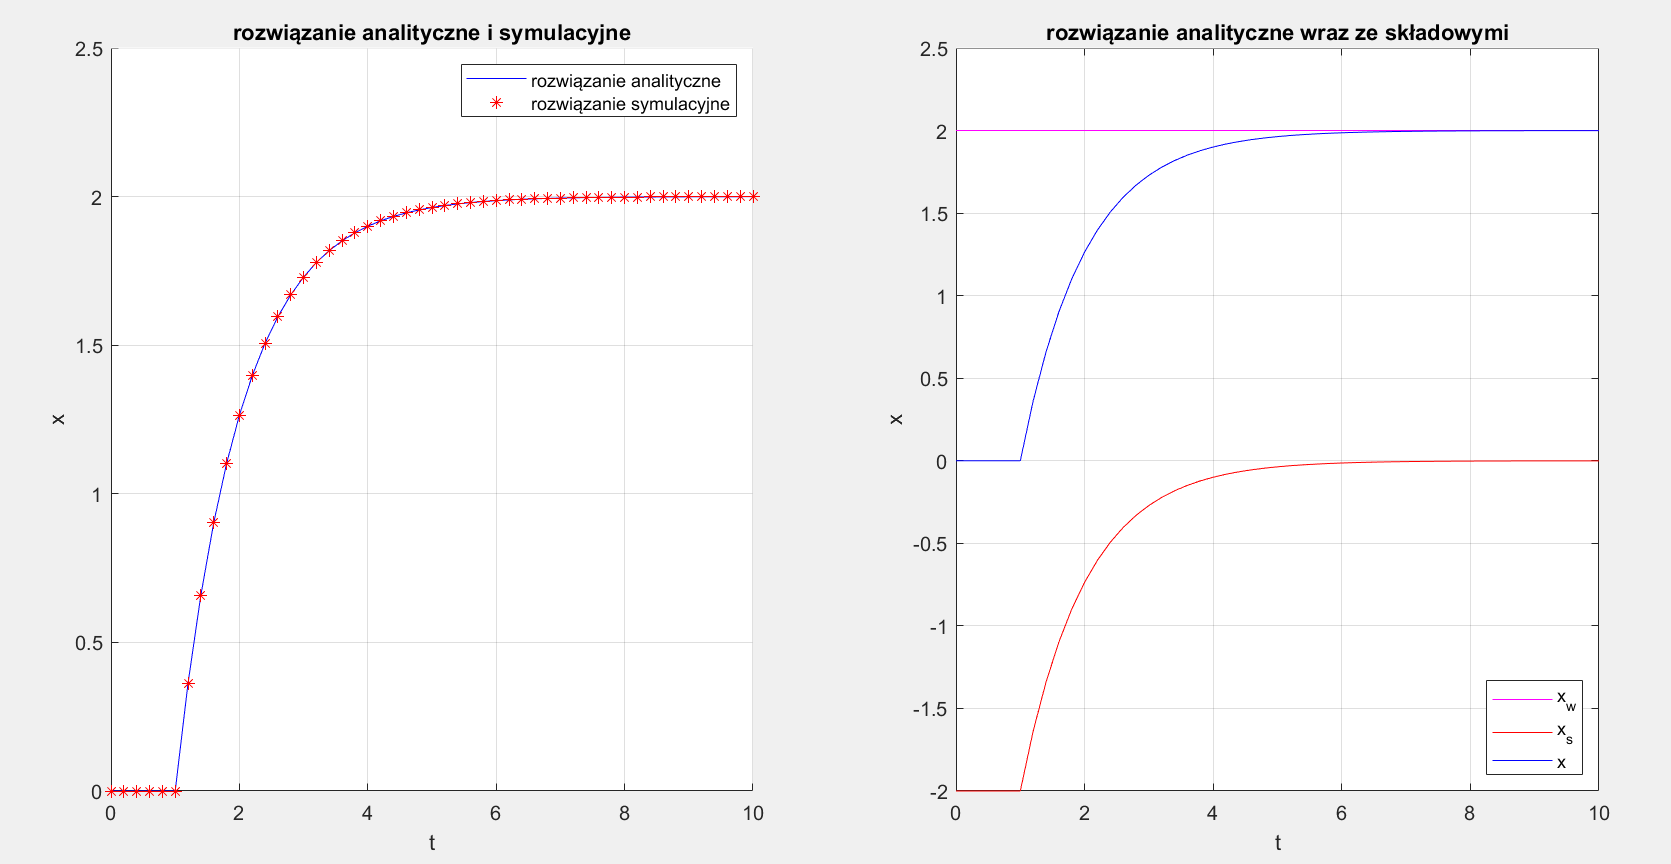
\includegraphics[width=\textwidth]{POPRAWAwykresC.png}
    \label{fig:my_label}
\end{figure}


\begin{flushleft}
d) Warunek początkowy $x(0)=2$\\
\end{flushleft}
Rozwiązanie analityczne, jego wykres wraz z wykresem składowych jego rozwiązania:\\
$$
x(t)=Ae^{-t}+2
$$
$$
2=A+2 \Rightarrow A=0
$$
$$
x(t)=2-\text{rozwiązanie szczególne}
$$
$$
x_s(t)=0, \  x_w(t)=2
$$
\newpage
Wykres dla rozwiązania analitycznego i symulacyjengo oraz wykres dla rozwiązania analitycznego wraz z składowymi:\\
\begin{figure}[h!]
    \centering
    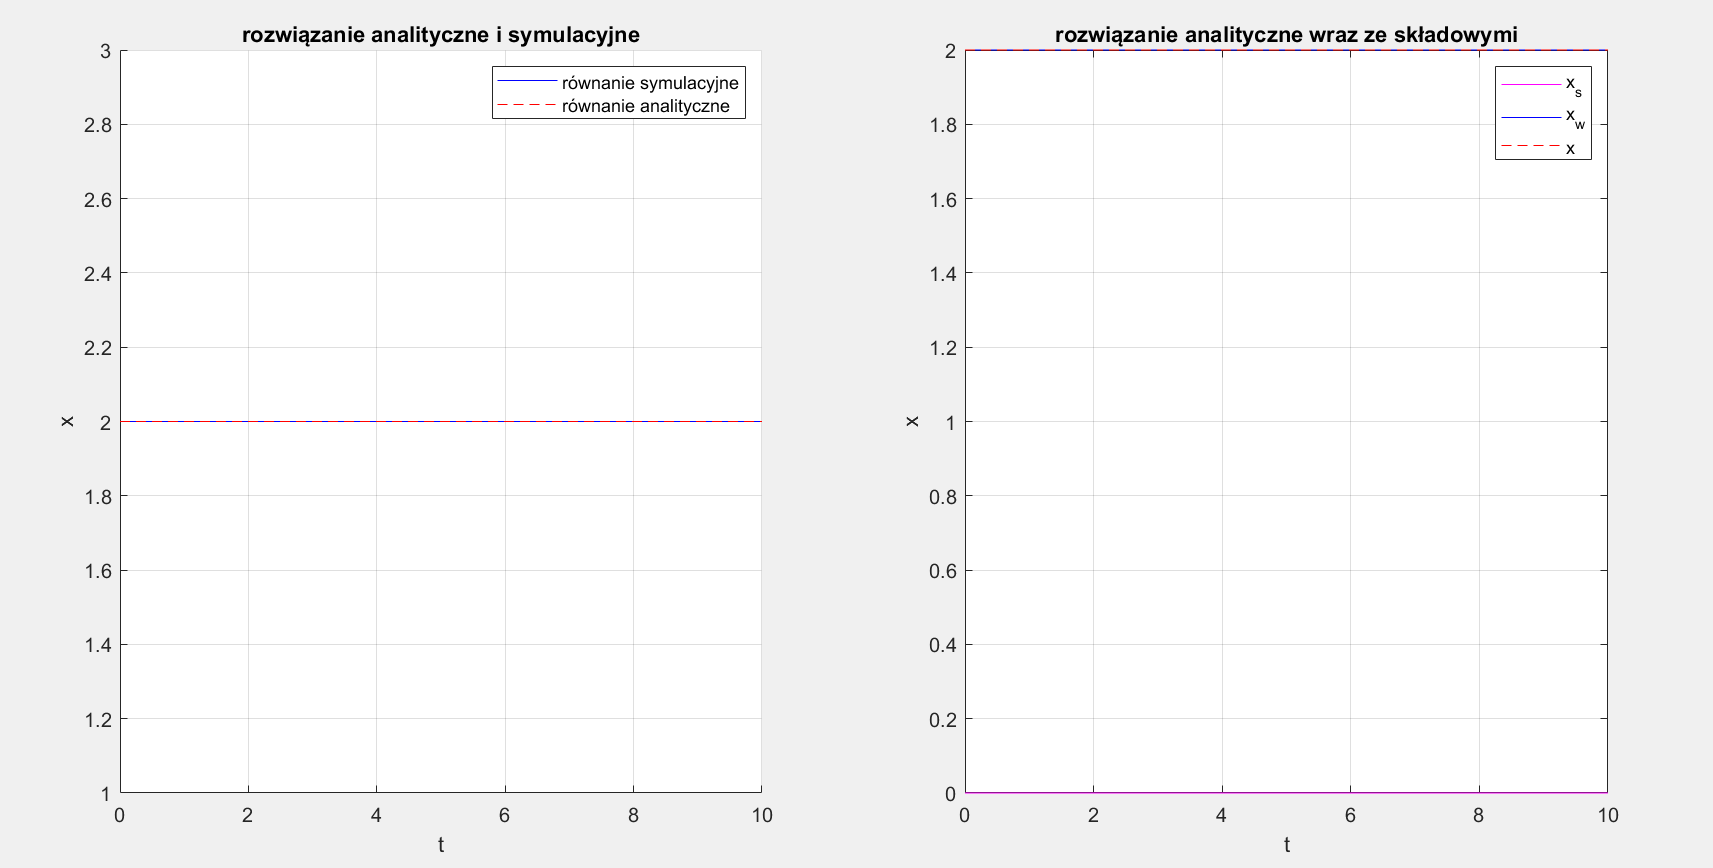
\includegraphics[width=\textwidth]{POPRAWAwykresD.png}
    \label{fig:my_label}
\end{figure}\\
Jak widać wykres jest linią prostą co oznacza ponieważ w równaniu szczególnym pozostało jedynie wymuszenie.

\section{Wnioski}
Z badań wynika żę wyniki uzyskane metodą analityczną oraz metądą symulacyjną są takie same. Podczas zadania przekonaliśmy się jak szybko i wygodnie za pomocą programu Simulink można wyliczyć równanie różniczkowe oraz zbadać jego wykres. 
\section{Załączniki}
\begin{figure}
    \centering
    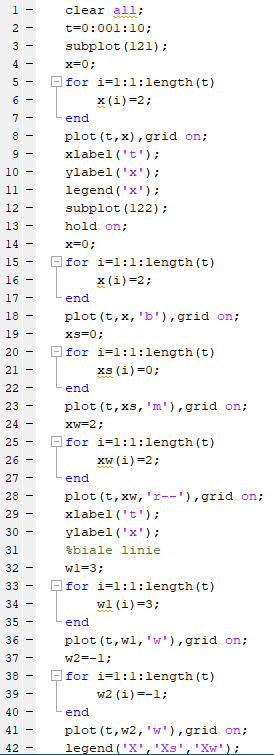
\includegraphics{kod1.png}
    \label{fig:my_label}
\end{figure}
\begin{figure}
    \centering
    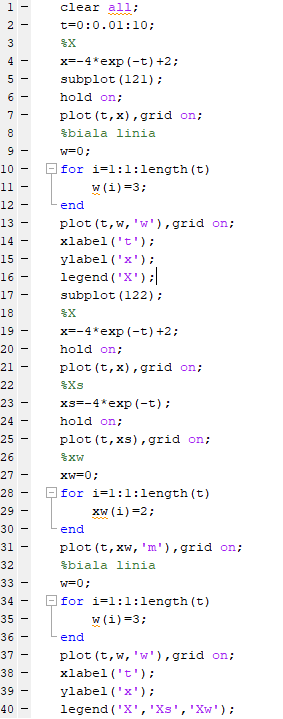
\includegraphics{kod2.png}
    \label{fig:my_label}
\end{figure}
\begin{figure}
    \centering
    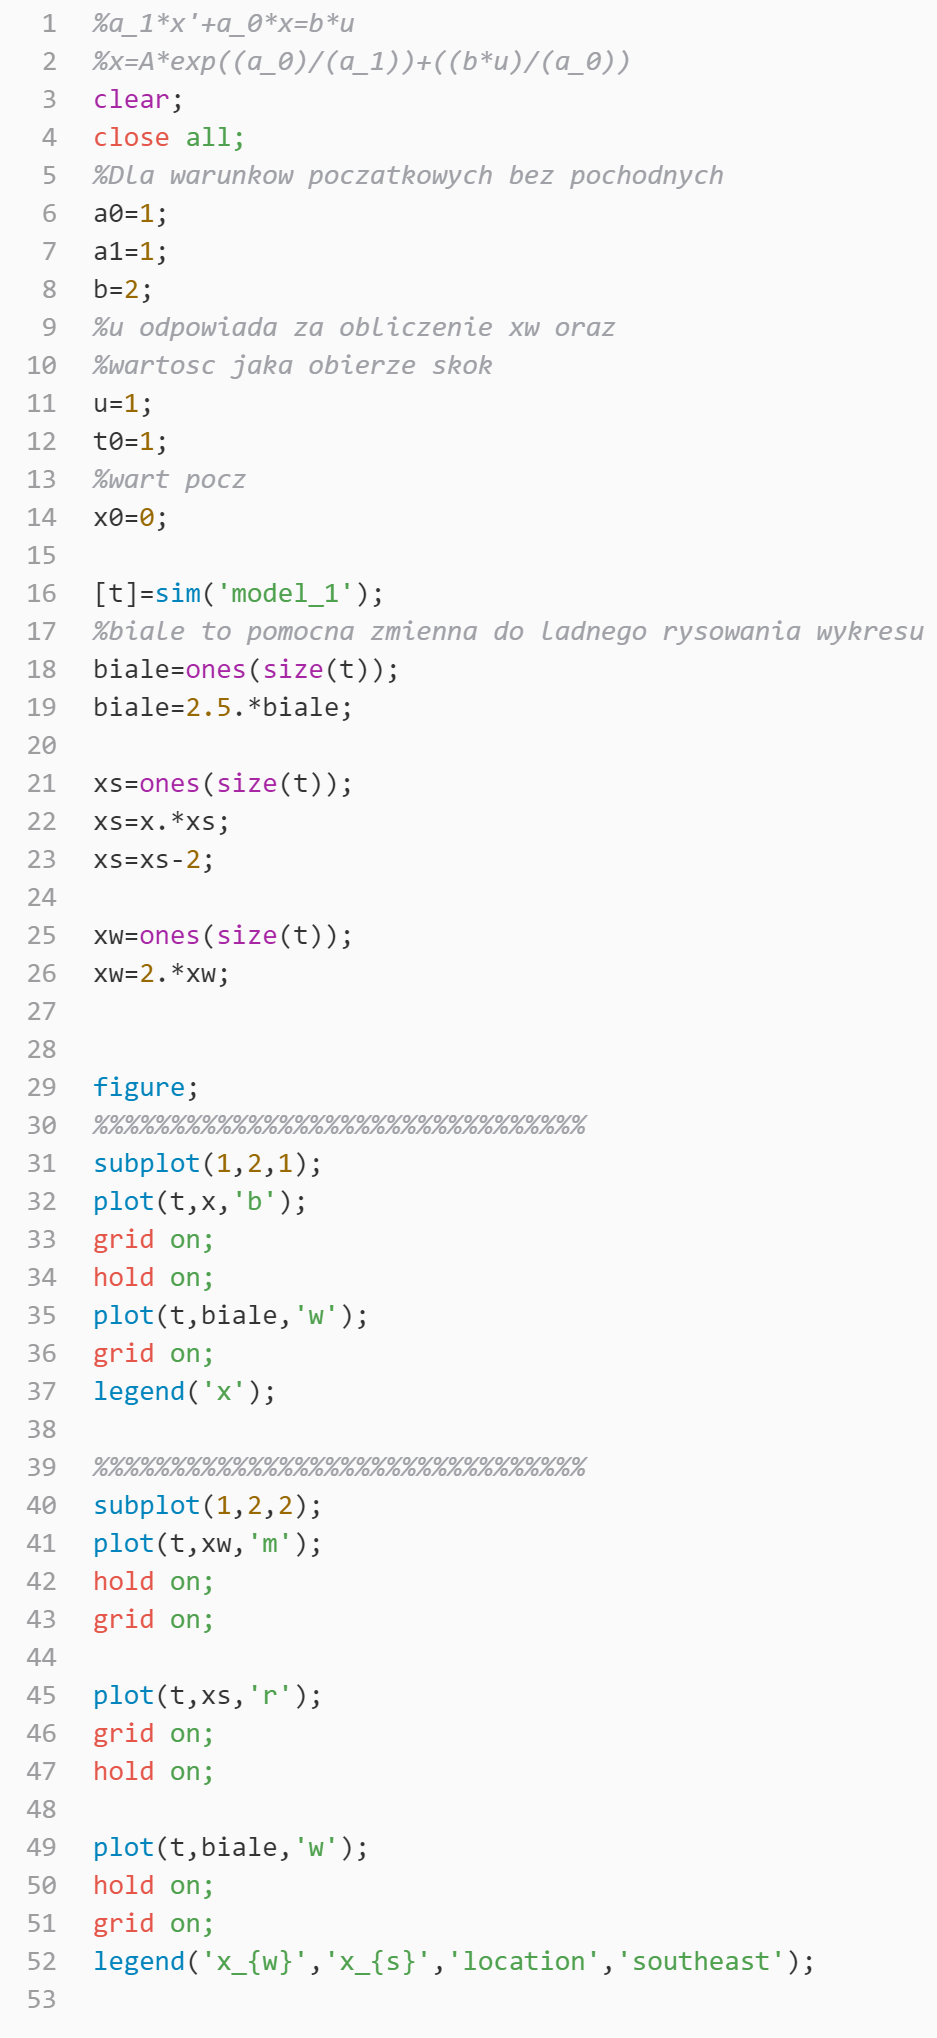
\includegraphics[width=0.6\textwidth]{kod_x_0.png}
    \label{fig:my_label}
\end{figure}
\begin{figure}
    \centering
    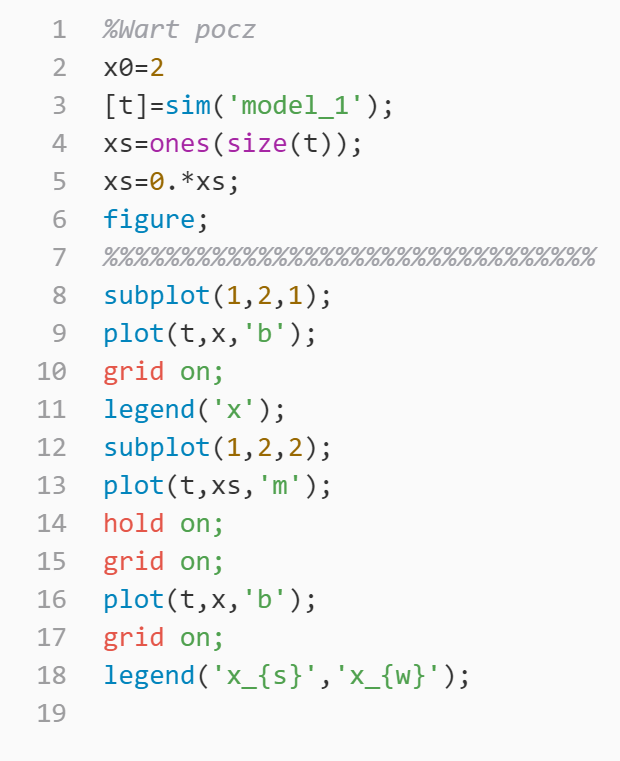
\includegraphics[width=0.6\textwidth]{kod_x_2.png}
    \label{fig:my_label}
\end{figure}
\end{document}
